\documentclass[11pt,a4paper]{article}
\usepackage{graphicx}
\usepackage{longtable}
\usepackage{float}
\usepackage{wrapfig}
\usepackage{rotating}
%\usepackage{a4wide}
\usepackage[normalem]{ulem}
\usepackage{amsmath}
\usepackage{textcomp}
\usepackage{marvosym}
\usepackage{wasysym}
\usepackage{amssymb}
\usepackage{hyperref}
%\usepackage[utf8]{inputenc}
%\usepackage[T1]{fontenc}
%\usepackage{polyglossia}
%\setmainlanguage[]{french}
\usepackage[top=30pt,bottom=50pt,left=48pt,right=46pt]{geometry}
\usepackage{listings}
\usepackage{svg}


\lstset{
    language=C++
  , frame=single
  , basicstyle=\scriptsize
  , keywordstyle=\color{blue}\bfseries
  , commentstyle=\color{red}
  , stringstyle=\color{magenta}\ttfamily
  , backgroundcolor=\color{black!5}
}

\usepackage[dvipsnames]{xcolor}
\usepackage{subfigure,tikz}
\usetikzlibrary{shadows,shadows.blur, trees,matrix,arrows,decorations}
\usetikzlibrary{decorations.pathmorphing, fadings, shapes, shapes.arrows, positioning, calc, shapes,fit}
\usepackage{fp}
\usepackage{pgfplots}
\tolerance=1000
\author{Xavier JUVIGNY}
\date{\today}
\title{Travaux dirigés n°1}

\newtheorem{definition}{Définition}
\newtheorem{theo}{Théorème}

\definecolor{verylightgray}{rgb}{0.95 0.95 1.0}

\definecolor{darkblue}{rgb}{0. 0. 0.4}

\begin{document}
\maketitle
\tableofcontents

\section{Produit matrice--matrice}

Soient $A$ et $B$ deux matrices définies à l'aide de deux couples de vecteurs $\left\{u_{A},v_{A}\right\}$ et 
$\left\{u_{B},v_{B}\right\}$ :
\[
\left\{
	\begin{array}{lcl}
	A & = & u_{A}.v_{A}^{T}\mbox{ soit } A_{ij} = u_{A_{i}}.v_{A_{j}} \\
	B & = & u_{B}.v_{B}^{T}\mbox{ soit } B_{ij} = u_{B_{i}}.v_{B_{j}}
    \end{array}
\right..
\]

On calcule le produit matrice--vecteur C=A.B à l'aide d'un produit matrice--matrice plein (complexité de $2.n^{3}$ opérations arithmétiques)
et on valide le résultat obtenu à l'aide de l'expression sous forme de produit tensoriel de $A$ et $B$ :
\[
\begin{array}{lclclcl}
C & = & A.B & = & \left(u_{A}.v_{A}^{T}\right).\left(u_{B}.v_{B}^{T}\right) & = &  u_{A}\left(v_{A}^{T}.u_{B}\right)v_{B}^{T}\\
 &=& u_{A}\left(v_{A}|u_{B}\right)v_{B}^{T} & = & \left(v_{A}|u_{B}\right)u_{A}.v_{B}^{T}
 \end{array}.
\]

Soit :
\[
C_{ij} = \left(v_{A}|u_{B}\right)u_{A_{i}}.v_{B_{j}},
\]
ce qui nécessite en tout $2.n+2.n^{2}$ opérations arithmétiques (dont $2.n$ opérations pour le produit scalaire).

On se propose, par étape, de paralléliser en mémoire partagée le produit matrice--matrice fourni dans le fichier \texttt{ProdMatMat.cpp}. 
L'exécutable pour tester le produit matrice-matrice est \texttt{TestProduitMatrix.exe} :

\begin{enumerate}
	\item Mesurez le temps de calcul du produit matrice--matrice donné en donnant en entrée diverses dimensions. Essayez en particulier de prendre pour dimension 1023, 1024 et 1025 (il suffit de passer la dimension en argument à l'exécution. Par exemple \verb@./TestProductMatrix.exe 1023@ testera le produit matrice-matrice pour des matrices de dimension 1023). En vous servant des transparents du cours, expliquez clairement les temps obtenus.
	
	\textbf{Réponse :} Pour \( n = 1024 \), le temps de calcul du produit de matrices est beaucoup plus long que pour \( n = 1023 \) et \( n = 1025 \). Cela se produit systématiquement pour des valeurs correspondant à des puissances de 2 supérieures à la taille de bloc (\textbf{block size}) du cache du processeur. Dans le cas de mon processeur, cette taille est de 64 octets.  

Ce problème s'explique par un alignement mémoire qui entraîne des conflits de cache constants. Comme \( 1024 \) est une puissance de 2, les adresses mémoire des éléments des matrices sont parfaitement alignées, ce qui peut rendre les accès moins efficaces en raison du \textbf{conflit de cache}. En revanche, pour \( n = 1023 \) et \( n = 1025 \), les accès ne suivent pas un schéma aussi rigoureusement aligné, ce qui réduit ces problèmes et permet d'obtenir de meilleures performances.
	
	\item \textbf{\color{blue}Première optimisation :} Permutez les  boucles en $i,j$ et $k$ jusqu'à obtenir un temps optimum pour le calcul du produit matrice--matrice (et après vous être persuadé que cela ne changera rien au résulat du calcul). Expliquez pourquoi la permutation des boucles optimale que vous avez trouvée
	est bien la façon optimale d'ordonner les boucles en vous servant toujours du support de cours.
	
	\textbf{Réponse :} L'ordre \( j, k, i \) est le plus efficace, car il fixe d'abord une colonne de \( B \),
	 puis une colonne de \( A \), et enfin parcourt les lignes de cette colonne de \( A \).
	Cette approche est optimale en raison de la façon dont les matrices sont stockées en mémoire sous la forme d'un
	vecteur unidimensionnel (\texttt{m\_arr\_coefs[row + col * nRows]}).
	Comme les éléments d'une même colonne sont contigus en mémoire, cet ordre de boucle permet de les accéder de manière séquentielle,
	exploitant ainsi la localité spatiale et réduisant les rechargements inutiles du cache.
	De plus, la matrice \( B \) est également accédée de manière contiguë, minimisant ainsi les erreurs de cache
	(\textbf{cache misses}). De cette façon, nous évitons les rechargements inutiles du cache et assurons un accès plus
	efficace aux données, améliorant ainsi de manière significative les performances du produit matriciel.

	\item \textbf{\color{blue}Première parallélisation :} A l'aide d'OpenMP, parallélisez le produit matrice--matrice. Mesurez le temps obtenu en variant le nombre de threads à l'aide de la variable d'environnement \texttt{OMP\_NUM\_THREADS}. Calculez l'accélération et le résultat obtenu en fonction du nombre de threads, commentez et expliquez clairement ces résultats. 
	
	\textbf{Réponse :} L'ajout de la directive \# pragma omp parallel for avant la boucle externe est suffisant pour une parallélisation initiale, car cela distribue les itérations de la boucle entre les threads, permettant à différentes parties de la multiplication de matrices d'être traitées simultanément. Cela se traduit par une réduction du temps d'exécution et une utilisation plus efficace des ressources informatiques disponibles.

	\begin{figure}[H]
		\centering
		\includegraphics[width=\textwidth]{parallel1.pdf}
		\caption{Speedup of matrix multiplication using OpenMP with varying thread counts.}
	\end{figure}

	\item Argumentez et donnez clairement la raison pour laquelle il est sûrement possible d'améliorer le résultat que vous avez obtenu.
	
	\textbf{Réponse :} 
	
	Il est nécessaire d'utiliser correctement la fonction \textbf{prodSubBlock} en parallélisant le calcul de la matrice dans des régions indépendantes. Cela permet d'optimiser l'utilisation du cache entre les processeurs, car chaque processeur travaille sur une partie spécifique de la mémoire, évitant ainsi de charger les mêmes données dans plusieurs caches. Par conséquent, il n'y a pas besoin de transférer les mêmes informations entre la mémoire principale et les caches à plusieurs reprises, ce qui diminue la latence d'accès à la mémoire et améliore considérablement les performances grâce à une meilleure gestion des ressources et un meilleur partage du travail.

	\item \textbf{\color{blue}Deuxième optimisation :} Pour pouvoir exploiter au mieux la mémoire cache, on se propose de transformer notre produit matrice--matrice "scalaire" en produit matrice--matrice par bloc (on se servira pour le produit "bloc--bloc" de la meilleure version \textbf{séquentielle} du produit matrice--matrice obtenu précédemment).

	L'idée est de décomposer les matrices $A,B$ et $C$ en sous-blocs matriciels :
	\[
	A = \left(
	\begin{array}{cccc}
	A_{11} & A_{12} & \ldots & A_{1N} \\
	A_{21} & \ddots &        & \vdots \\
	\vdots &        & \ddots & \vdots \\
	A_{N1} &        &        & A_{NN}
	\end{array}
	\right),
	B = \left(
	\begin{array}{cccc}
	B_{11} & B_{12} & \ldots & B_{1N} \\
	B_{21} & \ddots &        & \vdots \\
	\vdots &        & \ddots & \vdots \\
	B_{N1} &        &        & B_{NN}
	\end{array}
	\right),
	C = \left(
	\begin{array}{cccc}
	C_{11} & C_{12} & \ldots & C_{1N} \\
	C_{21} & \ddots &        & \vdots \\
	\vdots &        & \ddots & \vdots \\
	C_{N1} &        &        & C_{NN}
	\end{array}
	\right),
	\]

où $A_{IJ},B_{IJ}$ et $C_{IJ}$ sont des sous--blocs possédant une taille fixée (par le programmeur ).

Le produit matrice--matrice se fait alors par bloc. Pour calculer le bloc $C_{IJ}$, on calcule :
\[
C_{IJ} = \sum_{K=1}^{N}A_{IK}.B_{KJ}.
\]

Mettre en {\oe}uvre ce produit matrice--matrice en séquentiel puis faire varier la taille des blocs jusqu'à obtenir un optimum.


\textbf{Réponse :} 
Pour la prochaine étape de parallélisation, nous allons utiliser le code suivant :

\begin{lstlisting}[caption={Parallélisation avec OpenMP}, label={lst:parallel}]
  for (int iRowBlkA = 0; iRowBlkA < A.nbRows; iRowBlkA += szBlock)
    for (int iColBlkB = 0; iColBlkB < B.nbCols; iColBlkB += szBlock)
      for (int iColBlkA = 0; iColBlkA < A.nbCols; iColBlkA += szBlock)
        prodSubBlocks(iRowBlkA, iColBlkB, iColBlkA, szBlock, A, B, C);
\end{lstlisting}

\item Comparer le temps pris par rapport au produit matrice--matrice "scalaire". Comment interprétez vous le résultat obtenu~?

\textbf{Réponse :} Les tests ont montré qu'en augmentant progressivement la taille des blocs lors de la multiplication matricielle, on améliore significativement les performances par rapport à la méthode scalaire, grâce à une meilleure exploitation du cache mémoire. En effet, des tailles de blocs faibles entraînent des accès discontinus aux données, alors qu'une taille de 64 optimise la réutilisation des informations en cache, réduisant ainsi le temps d'exécution. Au-delà de cette valeur, les gains se stabilisent, indiquant que la taille de bloc optimale pour cette processeur se situe autour de 64.

\begin{figure}[H]
	\centering
	\includegraphics[width=\textwidth]{sizeBlock.pdf}
	\caption{Performance vs Block Size (Matrix Size = 2048)}
\end{figure}

\item \textbf{\color{blue}Parallélisation du produit matrice--matrice par bloc }: \`A l'aide d'OpenMP, parallélisez le produit matrice--matrice par bloc puis mesurez l'accélération parallèle en fonction du nombre de threads. Comparez avec la version scalaire parallélisée. Comment expliquez vous ce résultat ?


Pour la prochaine étape de parallélisation, nous allons utiliser le code suivant :
\begin{lstlisting}[caption={Parallélisation avec OpenMP}, label={lst:parallel}]
#pragma omp parallel
{
  #pragma omp for collapse(2) schedule(dynamic)
  for (int iRowBlkA = 0; iRowBlkA < A.nbRows; iRowBlkA += szBlock)
    for (int iColBlkB = 0; iColBlkB < B.nbCols; iColBlkB += szBlock)
      for (int iColBlkA = 0; iColBlkA < A.nbCols; iColBlkA += szBlock)
        prodSubBlocks(iRowBlkA, iColBlkB, iColBlkA, szBlock, A, B, C);
}
\end{lstlisting}

Ce code utilise la directive \texttt{\#pragma omp parallel} pour créer une région parallèle, et la directive \texttt{\#pragma omp for collapse(2) schedule(dynamic)} pour paralléliser les deux premières boucles imbriquées. Cette approche permet de combiner les itérations des deux boucles afin de répartir plus efficacement la charge de travail entre les threads. En assignant à chaque thread un sous-bloc indépendant de la matrice, on optimise l'utilisation du cache en évitant de charger plusieurs fois les mêmes données dans différents caches. Ainsi, chaque processeur gère des portions spécifiques de la mémoire, ce qui améliore globalement la performance du calcul en réduisant les accès redondants en mémoire.


\begin{figure}[H]
	\centering
	\includegraphics[width=\textwidth]{SpeedUp.pdf}
	\caption{Speedup of matrix multiplication using OpenMP with varying thread counts.}
	\label{fig:speedup}
\end{figure}

\item \textbf{\color{blue}{Comparaison avec blas}}: Comparez vos résultat avec l'exécutable \texttt{produit\_matmat\_blas.exe} qui utilise un produit matrice-matrice 
                                                     optimisé. Quel rapport de temps obtenez vous ? Quelle version est la meilleure selon vous ?

\textbf{Réponse: }

Notre multiplication par blocs optimisée a atteint une performance maximale d'environ 20000 MFLOPS pour une matrice de taille 2048, tandis que l'implémentation BLAS réalise le même calcul en obtenant environ 219430 MFLOPS. Cela correspond à un gain d’environ 11 fois en faveur de BLAS, ce qui démontre que, malgré les améliorations significatives apportées par l’algorithme par blocs (notamment grâce à une meilleure exploitation du cache), l'optimisation poussée et les techniques de parallélisme, vectorisation et gestion mémoire de BLAS en font la version la plus performante pour la multiplication matricielle.
\end{enumerate}

\section{Parallélisation MPI}

Ecrivez en langage C les programmes suivants.

\subsection{Circulation d'un jeton dans un anneau}

Ecrivez un programme tel que :
\begin{enumerate}
	\item le processus de rang zéro initialise un jeton à 1 puis l'envoie au processus de rang un;
	\item le processus de rang un reçoit le jeton, l'incrémente de un puis l'envoie au processus de rang deux;
	\item \ldots
	\item le processus de rang $p$ reçoit le jeton, l'incrémente de un puis l'envoie au processus de rang $p+1$ ($0<p<nbp-1$);
	\item \ldots
	\item le processus de rang $\mbox{nbp}-1$ reçoit le jeton, l'incrémente de un et l'envoie au processus de rang zéro;
	\item le processus de rang zéro reçoit le jeton du processus $\mbox{nbp}-1$ et l'affiche à l'écran.
\end{enumerate}

\subsection{Calcul tr\`es approch\'e de pi}

On veut calculer la valeur de pi à l'aide de l'algorithme stochastique suivant :
\begin{itemize}
\item on considère le carré unité
$\left[-1;1\right]\times \left[-1;1\right]$ dans lequel on inscrit le cercle unité de centre $(0,0)$ et de rayon $1$;
\item on génère des points aléatoirement dans le carré unité;
\item on compte le nombre de points générés dans le carré qui sont aussi dans le cercle;
\item soit $r$ ce nombre de points dans le cercle divisé par le nombre de points
  total dans le carré, on calcule alors pi comme $\pi = 4.r$.
\end{itemize}

Remarquez que l'erreur faite sur pi décroit quand le nombre de points générés augmente.

\begin{center}
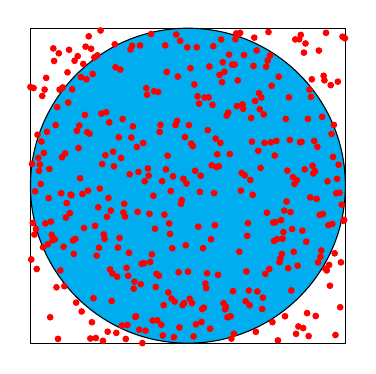
\begin{tikzpicture}[scale=2]
\draw[color=black,fill=cyan] (0,0) circle (1);
\draw[color=black] (-1,-1) -- (-1,1) -- (1,1) -- (1,-1) -- cycle;
\draw[red] plot[only marks, mark=*, mark size=0.5, domain=-1:1, samples=400] (\x,{rnd*2-1});
\end{tikzpicture}
\end{center}

Couper l'itération de boucle en plusieurs morceaux pouvant être exécutés par différentes tâches
simultanément:
\begin{itemize}
\item chaque tâche exécute sa portion de boucle;
\item chaque tâche peut exécuter son travail sans avoir besoin d'information des autres tâches (indépendance des données);
\item la tâche maître (que le programmeur aura choisi parmi ses tâches) reçoit le résultat des autres
tâches à l'aide d'échanges de message point à point;
\item utiliser l'échange de message global adéquat pour obtenir le résultat final.
\end{itemize}

Mesurez le temps mis par les deux versions (séquentiel et parallèle) et calculez 
l'accélération obtenue. Est-ce cohérent avec votre machine (cf. \verb|lscpu| ou gestionnaire de tâches) ?

\begin{center}
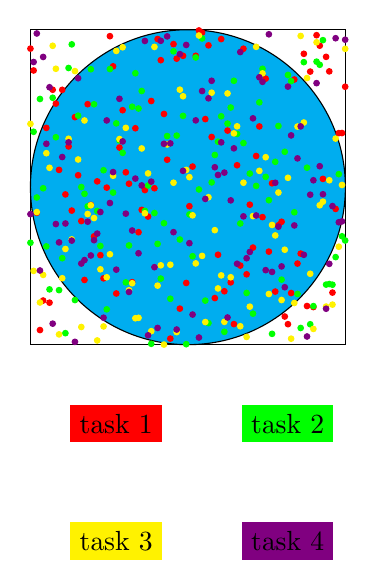
\begin{tikzpicture}[scale=2]
\draw[color=black,fill=cyan] (0,0) circle (1);
\draw[color=black] (-1,-1) -- (-1,1) -- (1,1) -- (1,-1) -- cycle;
\draw[color=red,fill=red] plot[only marks, mark=*, mark size=0.5, domain=-1:1, samples=100] (\x,{rnd*2-1});
\draw[color=green,fill=green] plot[only marks, mark=*, mark size=0.5, domain=-1:1, samples=100] (\x,{rnd*2-1});
\draw[color=yellow, fill=yellow] plot[only marks, mark=*, mark size=0.5, domain=-1:1, samples=100] (\x,{rnd*2-1});
\draw[color=violet, fill=violet] plot[only marks, mark=*, mark size=0.5, domain=-1:1, samples=100] (\x,{rnd*2-1});
\draw (-0.75,-1.5) node[right,rectangle,fill=red] (t1) {task 1};
\draw node[right, right=of t1, rectangle,fill=green] (t2) {task 2};
\draw node[right, below=of t1, rectangle, fill=yellow] (t3) {task 3};
\draw node[right, right=of t3, rectangle, fill=violet] (t4) {task 4};
\end{tikzpicture}
\end{center}

\fbox{
\begin{minipage}{\textwidth}
\underline{Le concept} : diviser le travail parmi les tâches disponibles en communicant des données à l'aide
d'appel à des fonctions d'envoi/réception point à point.

\end{minipage} }

\pagebreak
\textbf{\textcolor{red}{A FAIRE}} : 
\begin{itemize}
\item Paralléliser en mémoire partagée le programme séquentiel en C à l'aide d'OpenMP

\begin{lstlisting}[language=C++, caption=Monte Carlo et OpenMP]
double approximate_pi(unsigned long nbSamples) {
unsigned long nbDarts = 0;

#pragma omp parallel
{
unsigned int seed = static_cast<unsigned int>(
	chrono::high_resolution_clock::now().time_since_epoch().count()
		+ omp_get_thread_num()
);
std::default_random_engine generator(seed);
std::uniform_real_distribution<double> distribution(-1.0, 1.0);

#pragma omp for reduction(+:nbDarts)
	for (unsigned long sample = 0; sample < nbSamples; ++sample) {
		double x = distribution(generator);
		double y = distribution(generator);
		if (x * x + y * y <= 1.0)
			nbDarts++;
	}
}

double ratio = static_cast<double>(nbDarts) / static_cast<double>(nbSamples);
return 4.0 * ratio;
}
\end{lstlisting}
	

\item Mesurez l'accélération obtenue en utilisant un nombre variable de coeurs de calcul

\begin{figure}[H]
	\centering
	\includegraphics[width=\dimexpr\textwidth]{sources/calcul_pi/plot.png}
	\caption{Monte Carlo - OpenMP with varying thread counts.}
\end{figure}


\item Paralléliser en mémoire distribuée le programme séquentiel en C à l'aide de MPI 

\begin{lstlisting}[language=C++, caption=Monte Carlo et MPI reduction]
int main(int argc, char* argv[])
{
    // Initialize MPI
    MPI_Init(&argc, &argv);
    MPI_Comm globComm;
    MPI_Comm_dup(MPI_COMM_WORLD, &globComm);

    // Get number of processes and current process rank
    int nbp, rank;
    MPI_Comm_size(globComm, &nbp);
    MPI_Comm_rank(globComm, &rank);

    // Distribute samples among processes
    unsigned long totalSamples = 100000000;
    if (argc > 1)
        totalSamples = std::stoul(argv[1]);
    unsigned long localSamples = totalSamples / nbp;

    // Each process performs its part of the simulation
    unsigned long localCount = 0;
    std::default_random_engine generator(static_cast<unsigned>(
        std::chrono::high_resolution_clock::now().time_since_epoch().count()) + rank);
    std::uniform_real_distribution<double> distribution(-1.0, 1.0);

    for (unsigned long i = 0; i < localSamples; ++i) {
        double x = distribution(generator);
        double y = distribution(generator);
        if (x * x + y * y <= 1.0)
            localCount++;
    }

    // Reduce local counts to compute the total count
    unsigned long globalCount = 0;
    MPI_Reduce(&localCount, &globalCount, 1, MPI_UNSIGNED_LONG, MPI_SUM, 0, globComm);

    // The root process computes and prints the final result
    if (rank == 0) {
        unsigned long usedSamples = localSamples * nbp;
        double pi = 4.0 * static_cast<double>(globalCount) / static_cast<double>(usedSamples);
        std::cout << "Approximation de pi = " << pi << std::endl;
    }

    MPI_Finalize();
    return EXIT_SUCCESS;
}
\end{lstlisting}

\item Mesurez l'accélération obtenue en utilisant un nombre variable de processus

\begin{figure}[H]
	\centering
	\includegraphics[width=\dimexpr\textwidth]{sources/calcul_pi/pi_MPI.png}
	\caption{Monte Carlo - MPI with varying thread counts.}
\end{figure}

\item Paralléliser en mémoire distribuée le programme séquentiel en Python à l'aide de mpi4py


\begin{lstlisting}[language=python, caption=Monte Carlo et MPI4PY reduction]

from mpi4py import MPI
import numpy as np
import time

comm = MPI.COMM_WORLD
rank = comm.Get_rank()
size = comm.Get_size()

nb_samples_total = 100_000_000

samples_per_process = nb_samples_total // size
reste = nb_samples_total % size
if rank < reste:
    samples_per_process += 1

if rank == 0:
    start_time = time.time()

x = 2.0 * np.random.random_sample(samples_per_process) - 1.0
y = 2.0 * np.random.random_sample(samples_per_process) - 1.0

local_count = np.sum(x*x + y*y < 1)

global_count = comm.reduce(local_count, op=MPI.SUM, root=0)

if rank == 0:
    approx_pi = 4.0 * global_count / nb_samples_total
    end_time = time.time()
    print(f"Temps pour calculer pi : {end_time - start_time} secondes")
    print(f"Pi vaut environ {approx_pi}")


\end{lstlisting}

\item Mesurez l'accélération obtenue en utilisant un nombre variable de processus

\begin{figure}[H]
	\centering
	\includegraphics[width=\dimexpr\textwidth]{sources/calcul_pi/PI_in_mpi4py.png}
	\caption{Monte Carlo - MPI4PY with varying thread counts.}
\end{figure}

\end{itemize}

\subsection{Diffusion d'un entier dans un réseau hypercube\textcolor{red}{$^{\star}$}}

On veut écrire un programme qui diffuse un entier dans un réseau de n{\oe}uds de calculs dont la topologie
est équivalente à celle d'un hypercube de dimension $d$ (et qui contient donc $2^{d}$ n{\oe}uds de calcul).

\begin{enumerate}
\item \'Ecrire un programme en C qui diffuse un entier dans un hyper cube de dimension 1 :
\begin{itemize}
\item la tâche 0 initialise un jeton à une valeur entière choisie par le programmeur et envoie cette valeur 
à la tâche 1; 
\item la tâche 1 reçoit la valeur du jeton de la tâche 0;
\item les deux tâches affichent la valeur du jeton.
\end{itemize}
\item Diffuser le jeton généré par la tâche 0 dans un hypercube de dimension 2 de manière que cette diffusion se fasse en un minimum
d'étapes (et donc un maximum de communications simultanées entre tâches).
\item Faire de même pour un hypercube de dimension 3.
\item \'Ecrire le cas général quand le cube est de dimension $d$. Le nombre d'étapes pour diffuser le jeton devra
être égal à la dimension de l'hypercube.
\item Mesurer l'accélération obtenue pour la diffusion d'un entier sur un tel réseau.
\end{enumerate}

\begin{center}
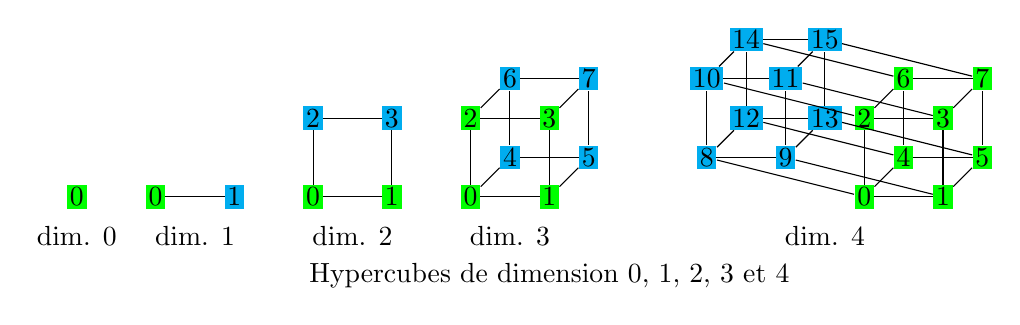
\begin{tikzpicture}
% Cube dimension 0
\draw (-4,0) node[fill=green,inner sep=1pt]{0};
\draw (-4,-0.5) node{dim. 0};
% Cube dimension 1
\draw (-3,0) node[fill=green,inner sep=1pt](cd1_0){0} -- (-2,0) node[fill=cyan,inner sep=1pt](cd1_1){1};
\draw (-2.5,-0.5) node{dim. 1};
% Cube dimension 2
\draw (-1,0) node[fill=green,inner sep=1pt](cd2_0){0} -- (0,0) node[fill=green,inner sep=1pt](cd2_1){1};
\draw (-1,1) node[fill=cyan,inner sep=1pt](cd2_2){2} -- (0,1) node[fill=cyan,inner sep=1pt](cd2_3){3};
\draw (cd2_0) -- (cd2_2) (cd2_1) -- (cd2_3);
\draw (-0.5,-0.5) node{dim. 2};
% Cube dimension 3
\draw (1,0) node[fill=green,inner sep=1pt](cd3_0){0} -- (2,0) node[fill=green,inner sep=1pt](cd3_1){1};
\draw (1,1) node[fill=green,inner sep=1pt](cd3_2){2} -- (2,1) node[fill=green,inner sep=1pt](cd3_3){3};
\draw (1.5,0.5) node[fill=cyan,inner sep=1pt](cd3_4){4} -- (2.5,0.5) node[fill=cyan,inner sep=1pt](cd3_5){5};
\draw (1.5,1.5) node[fill=cyan,inner sep=1pt](cd3_6){6} -- (2.5,1.5) node[fill=cyan,inner sep=1pt](cd3_7){7};
\draw (cd3_0) -- (cd3_2) (cd3_1) -- (cd3_3);
\draw (cd3_4) -- (cd3_6) (cd3_5) -- (cd3_7);
\draw (cd3_0) -- (cd3_4) (cd3_1) -- (cd3_5) (cd3_2)--(cd3_6) (cd3_3)--(cd3_7);
\draw (1.5,-0.5) node{dim. 3};
% Cube de dimension 4
\draw (6,0) node[fill=green,inner sep=1pt](cd4_0){0} -- (7,0) node[fill=green,inner sep=1pt](cd4_1){1};
\draw (6,1) node[fill=green,inner sep=1pt](cd4_2){2} -- (7,1) node[fill=green,inner sep=1pt](cd4_3){3};
\draw (6.5,0.5) node[fill=green,inner sep=1pt](cd4_4){4} -- (7.5,0.5) node[fill=green,inner sep=1pt](cd4_5){5};
\draw (6.5,1.5) node[fill=green,inner sep=1pt](cd4_6){6} -- (7.5,1.5) node[fill=green,inner sep=1pt](cd4_7){7};
\draw (cd4_0) -- (cd4_2) (cd4_1) -- (cd4_3);
\draw (cd4_4) -- (cd4_6) (cd4_5) -- (cd4_7);
\draw (cd4_0) -- (cd4_4) (cd4_1) -- (cd4_5) (cd4_2)--(cd4_6) (cd4_3)--(cd4_7);
\draw (4,0.5) node[fill=cyan,inner sep=1pt](cd4_8){8} -- (5,0.5) node[fill=cyan,inner sep=1pt](cd4_9){9};
\draw (4,1.5) node[fill=cyan,inner sep=1pt](cd4_10){10} -- (5,1.5) node[fill=cyan,inner sep=1pt](cd4_11){11};
\draw (4.5,1) node[fill=cyan,inner sep=1pt](cd4_12){12} -- (5.5,1) node[fill=cyan,inner sep=1pt](cd4_13){13};
\draw (4.5,2) node[fill=cyan,inner sep=1pt](cd4_14){14} -- (5.5,2) node[fill=cyan,inner sep=1pt](cd4_15){15};
\draw (cd4_8) -- (cd4_10) (cd4_9) -- (cd4_11);
\draw (cd4_12) -- (cd4_14) (cd4_13) -- (cd4_15);
\draw (cd4_8) -- (cd4_12) (cd4_9) -- (cd4_13) (cd4_10)--(cd4_14) (cd4_11)--(cd4_15);
\draw (cd4_0) -- (cd4_8) (cd4_1) -- (cd4_9) (cd4_2) -- (cd4_10) (cd4_3) -- (cd4_11) (cd4_4) -- (cd4_12) (cd4_5) -- (cd4_13) (cd4_6) -- (cd4_14) (cd4_7) -- (cd4_15);
\draw (5.5,-0.5) node{dim. 4};
\draw (2,-1) node{Hypercubes de dimension 0, 1, 2, 3 et 4};
\end{tikzpicture}
\end{center}


\end{document}
